\documentclass{beamer}

\usetheme{Warsaw}

\usepackage[utf8]{inputenc}
\usepackage[frenchb]{babel}
\usepackage[T1]{fontenc}
\usepackage{amsmath}
\usepackage{hyperref}
\usepackage{comment} 
\usepackage{graphicx}
\usepackage[linesnumbered]{algorithm2e}

\usepackage{tikz}
\usetikzlibrary{arrows}

\pdfcompresslevel0

\usepackage{color}

\addtobeamertemplate{footline}{\hfill\insertframenumber/\inserttotalframenumber

\hspace{10em}\\}

\usepackage{listings}

\title{Programmation générique basée sur les classes combinatoires}
\author{Marwan Ghanem - Charles Huyghues-Despointes}
\date{\today}

% slides number
\defbeamertemplate*{footline}{shadow theme}
{%
  \leavevmode%
  \hbox{
    \begin{beamercolorbox}[wd=.5\paperwidth,ht=2.5ex,dp=1.125ex,leftskip=.3cm plus1fil,rightskip=.3cm]{author in head/foot}%
    \usebeamerfont{author in head/foot}\insertframenumber\,/\,\inserttotalframenumber\hfill\insertshortauthor
  \end{beamercolorbox}%
  \begin{beamercolorbox}[wd=.5\paperwidth,ht=2.5ex,dp=1.125ex,leftskip=.3cm,rightskip=.3cm plus1fil]{}%
    \usebeamerfont{title in head/foot}\insertshorttitle%
  \end{beamercolorbox}}%
  \vskip0pt%
}

\beamertemplatenavigationsymbolsempty


\begin{document}

\maketitle




\begin{frame}{Objectif}

\begin{itemize}
\item Spécifier les classes combinatoires simples
\item Représenter les classes ( structure arborescente )
%%\item faire un lien entre les grammaires génératives et l'analyse combinatoire
\item Enumérer les objets par taille
\end{itemize}

\end{frame}





\begin{frame}{Rappel de combinatoire analytique}
\begin{definition}
\emph{Classe combinatoire :} \\
Ensemble fini tel que : \\
\begin{itemize}
\item on a une fonction taille sur ses éléments
\item la taille d'un élément est positive et finie
\end{itemize}

On appellera Z la classe contenant un seul élément de taille 1.
\end{definition}
\begin{block}{Exemple : les arbres binaires}
\begin{itemize}
\item $B = Z + Z \times B \times B$ \\
Z sert à dénombrer,
ici on dénombre les feuilles, mais aussi les noeuds internes
%%\item $ B = Leaf * <1> + B * B * <1> $\\
%%Séparation de ce qu'on compte et du terminal Leaf
\end{itemize}
\end{block}
\end{frame}





\begin{comment}

\begin{frame}{Rappel d'analyse combinatoire}

Operations usuelles
\begin{itemize}
\item Union disjointe ( $C + B$ )
\item Produit cartésien ( $C \times B$ )
\item Séquence ( $Seq(C)$ )
\item MSet ( $MSet(C)$ )
\item PSet ( $PSet(C)$ )
\item Cycle ( $Cyc(C)$ )
\end{itemize}
%%%\medskip
%%\begin{figure}[h]
%%  \centering
%%  \includegraphics[scale=0.6]{schemaOjacare.png}
%%  \caption{La génération de code d'O'Jacaré}
%%\end{figure}

\end{frame}

\end{comment}



\begin{frame}{Vers un encodage des classes combinatoires }
Trouver une grammaire simple pour encoder les classes combinatoire. \newline
\begin{itemize}
\item
\begin{tabbing}
\textbf{Classe combinatoire :} \\
\hspace{0.5cm} \= \kill
\> M = Z + Z $\times$ M $\times$ M + Z $\times$ M \\  %%je modifie ici on avait mis * a place de times
\end{tabbing}


\item
\begin{tabbing}
\textbf{Notre Grammaire :} \\
\hspace{0.5cm} \= \kill
\> M ::= Leaf * <1> + M * M * <1> + M * <1>; \\
\end{tabbing}
\end{itemize} 

\end{frame}




\begin{comment}


\begin{frame}{Vers un encodage des classe combinatoires}
  
\begin{tabular}{|l|c|c|c|c|}
\hline
\emph{Nom} & \emph{Analyse combinatoire} & \emph{Notre grammaire} \\
\hline\hline
Union disjointe & a + b & a + b * <0>\\\hline
Produit cartésion & a $\times$ b & a * b * <0>\\\hline
Séquence & Seq( a ) & SEQ( a ) * <0> \\\hline
MSet & MSet( a )  & SET( a ) * <0> \\\hline
Produit commutatif & a \& b & a \& b \\\hline
Augment de taille & a $\times Z^{n}$ & a * <n> \\\hline
PSet  & PSet( a )  & $\times$ \\\hline
Cycle  & Set( a )  & $\times$ \\\hline
\end{tabular} 

\end{frame}





\begin{frame}{Vers un encodage des classes combinatoires}
Des nouveautés introduites :
\begin{itemize}
\item le produit commutatif
\item l'associativité ( < -1 > )
\end{itemize}
$\rightarrow$ la simplification du MSet et du Seq
\end{frame}

\end{comment}


\begin{frame}{Algorithme de Generation}
  \scalebox{0.8}[0.65]{
  \begin{algorithm}[H]
  %%\algsetup{linenosize=\tiny}
   \KwResult{Genere tous les arbres de le taille demande}
   addToTable(constructers)\;
   start = 0\;
   \While{true}{
   List newList\;
   List list = mainList.get(start)\;
   taille = list.length\;
   i = 0\;
   sort(list)\;
   \While{i < taille}{
    Node tmp = list.get(i)\;
    taille = tmp.getFils().length\;
    \For{$j\leftarrow 0$ \KwTo $taille$}{
      \For{$j\leftarrow 0$ \KwTo $constructers.length$}{
       ArrayList <Node> t = tmp.AddLevel(constructers.get(z))\;
       addList(t, newList)\;    
      }
    }
    }
    \eIf{$newList.length$ \eq $0$}{
      break
    }{
    start++\;
   }
  }
  \end{algorithm}
  }
\end{frame}

\begin{frame}{Derollement d'algorithme}
\begin{tabbing}
\textbf{Grammaire :} \\
\hspace{0.5cm} \= \kill
\hspace{0.5cm} 
\> M ::= Leaf * <1> + M * <1> + M * M * <1>; \\
\end{tabbing}
\textbf{Completers :} \\
\begin{figure}[h]
\centering
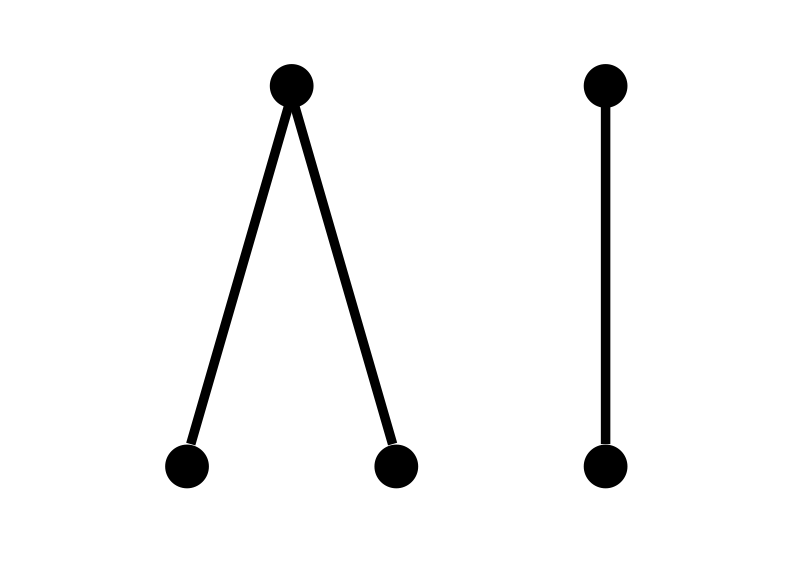
\includegraphics[scale=0.2]{const.png}
\end{figure}
\end{frame}


\begin{frame}{Derollement d'algorithme II}
\textbf{Generation 1:}\\
\begin{itemize}
\item  Avec Arbre unaire
\begin{figure}[h]
  \centering
  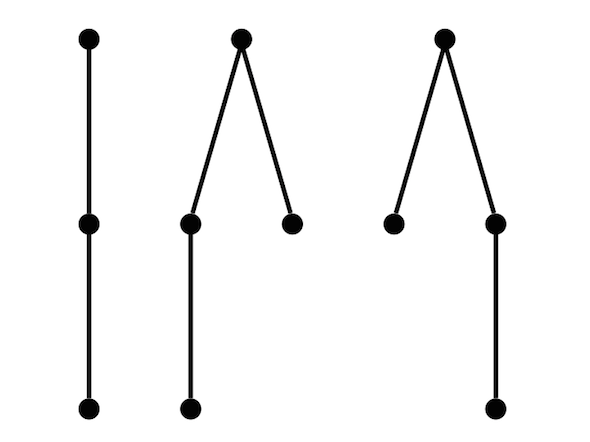
\includegraphics[scale=0.17]{gen1-1.png}
\end{figure}
\item Avec Arbre binare
\begin{figure}[h]
  \centering
  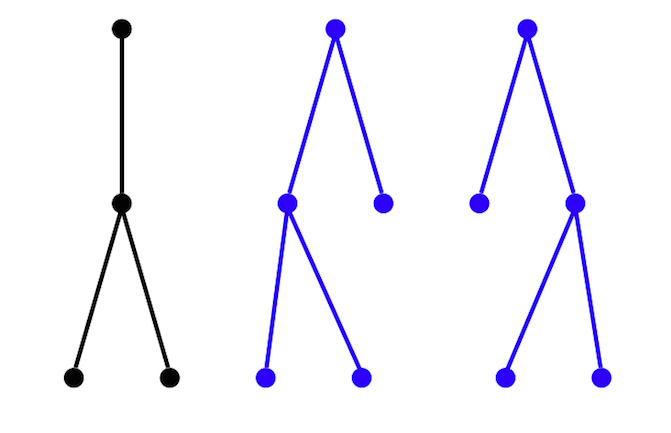
\includegraphics[scale=0.17]{gen1-2.png}
\end{figure}
\end{itemize}
\end{frame}



\begin{frame}{Derollement d'algorithme III}
\textbf{Generation 2:}\\
\begin{itemize}
\item  Avec Arbre unaire
\begin{figure}[h]
  \centering
  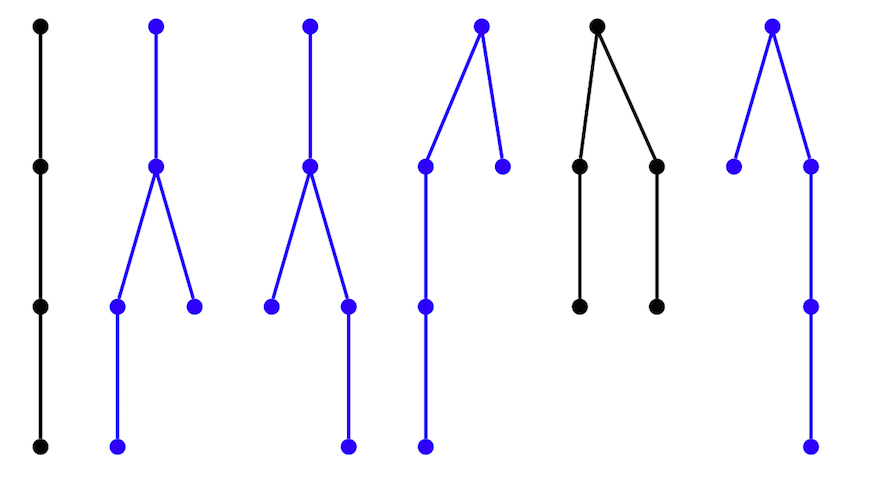
\includegraphics[scale=0.17]{gen2-1.png}
\end{figure}
\item Avec Arbre binare
\begin{figure}[h]
  \centering
  
\includegraphics[scale=0.17]{gen2-2.png}
\end{figure}
\end{itemize}
\end{frame}


\begin{frame}{Derollement d'algorithme IV}
\textbf{Generation 3:}\\
\begin{itemize}
\item  Avec Arbre unaire
\begin{figure}[h]
  \centering
  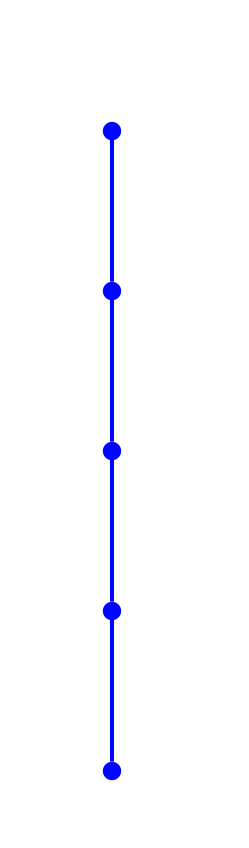
\includegraphics[scale=0.17]{gen3-1.png}
\end{figure}
\end{itemize}
\text{Nombre d'arbre trouve au fin : 9}
\end{frame}



\begin{frame}{Exemple: Partition et compostion d'entiers}
\begin{tabbing}
\hspace{1cm} \= \kill
\> \textbf{Composition et partition de 4}\\
\hspace{5cm} \= \kill
Composition \> Partition \\ 

$ 1 + 1 + 1 + 1 $ \> $ 1 +1 +1 +1 $\\
$ 1 + 1 + 2 $ \> $ 1 + 1 + 2 $\\
$ 1 + 2 + 1 $ \\
$ 2 + 1 + 1 $ \\
$ 2 + 2 $ \> $ 2 + 2 $ \\
$ 1 + 3 $ \> $ 1 + 3 $\\
$ 3 + 1 $ \\
$ 4 $ \> $ 4 $\\
\end{tabbing}
\end{frame}

\begin{frame}{Exemple: Partition et composition d'entiers}
\textbf{Composition :}\\
\begin{itemize}
\item
\begin{tabbing}
Classe combinatoire : \\
\hspace{0.5cm} \= \kill
\> C = Seq(Seq$_{>0}$(Z)) \\
\end{tabbing}
\item
\begin{tabbing}
Notre Grammaire : \\
\hspace{0.5cm} \= \kill
\hspace{0.5cm} 
\> P ::= Leaf * <1> + SEQ(E) * <1>; \\
\> E ::= Leaf * <1> + SEQ(E) * <-1>; \\
\end{tabbing}
\end{itemize} 
\textbf{Partition :}
\begin{itemize}
\item
\begin{tabbing}
Classe combinatoire : \\
\hspace{0.5cm} \= \kill
\> C = Set(Seq$_{>0}$(Z)) \\
\end{tabbing}
\item
\begin{tabbing}
Notre Grammaire : \\
\hspace{0.5cm} \= \kill
\hspace{0.5cm} 
\> P ::= Leaf * <1> + SET(E) * <1>; \\
\> E ::= Leaf * <1> + SEQ(E) * <-1>; \\
\end{tabbing}
\end{itemize} 
\end{frame}

\begin{frame}{Exemple: Partition et composition d'entiers}
ARBRES DE LA PARTITION DE 4
\end{frame}

\begin{frame}{Bilan}
\begin{itemize}
\item Prise en charge des opérateurs d'union, produit, séquence et multiSet
\item Trouver un truc à dire
\item Lien entre la combinatoire analytique et les grammaires génératives
\end{itemize}
\end{frame}



\begin{frame}{Et après \ldots}
\begin{itemize}
\item extension de la grammaire : PowerSet, Cycle,...
\item Génération automatique de code
\item Problème de reconnaissance de forme.
\end{itemize}
\end{frame}
%% \begin{frame}{Bibliographie}
  
%%   \begin{thebibliography}{9}
%%   \bibitem{amato2013localizing}
%%     Amato, Gianluca and Scozzari, Francesca,
%%     \emph{Localizing widening and narrowing}.
%%     Static Analysis, Springer.
%%     pages 25--42,
%%     2013.

%%   \bibitem{halbwachs2012decreasing}
%%     Halbwachs, Nicolas and Henry, Julien,
%%     \emph{When the decreasing sequence fails}.
%%     Static Analysis, Springer.
%%     pages 198--213,
%%     2012.
%%   \end{thebibliography}

%% \end{frame}

\end{document}

